\section{Introduction}
% Introduction 
% <<<
The Stokes equations \eqref{unsteady_stokes}, which are solved for an incompressible Navier-Stokes flow,
assume the Reynolds number is $Re \ll 1$ and thus advective processes are neglible in comparison to viscous processes.
The nonlinear term of the Navier-Stokes equations are then neglected, resulting in a far more numerically tractable set of equations.
The goal here is to derive and implement a linear Stokes flow solver, which can then be used as a component of a Navier-Stokes solver,
described in the next chapter.
We will solve, in particular, the steady-state form \eqref{steady_stokes}.
Due to this simplification, the Steady stokes equations \eqref{steady_stokes}, repeated here:
\begin{align*}
    -\nu\Delta u + \nabla p = \rho g, \quad \nabla\cdot u = 0,
\end{align*}
form a constrained linear equation. As we saw in section \ref{pressure_derivation}, the pressure term $p$ is a Lagrange multiplier introduced
with the constraint $\nabla\cdot u = 0$.

\subsection{The lid-driven cavity flow problem}
A standard test case in computational fluid dynamics is the \textit{lid-driven cavity flow} problem.
We let the domain be is $\Omega = [-1,1]^2$ and define a Dirichlet boundary condition:
\begin{equation}\label{lid_driven_boundary_condition}
    \left.u\right|_\Gamma = u_\Gamma(x,y) =
    \left\{\begin{array}{lr}
        \left(1, 0\right)^T &\text{if $y = 1$,}\\
        \left(0, 0\right)^T &\text{otherwise}.\\
        \end{array}\right.
\end{equation}
We will use a finite element method to solve the steady Stokes flow \eqref{steady_stokes} with this domain and boundary condition. A highly viscous incompressible
fluid under these conditions will form a single stable vortex.

\section{Attempting solution by an iterative pressure update}
% <<<
Since the steady Stokes equations are a linearly constrained vector Poisson equation,
it would be convenient to use a solution method which trivially extends our already-implemented Poisson solver.
One idea is to define a coupled system of equations replacing the constrained equation \eqref{steady_stokes}, resulting in an initial boundary value problem
in auxilliary parameter $\gamma$:
\begin{equation}
\begin{split}
    -\nu\Delta u &= -\nabla p_*,\\
    \Part{p_*}{\gamma} &= -C\nabla\cdot u,\\
    \text{with \quad} \left.u\right|_\Gamma &= u_\Gamma,\quad u(\hat{x}, 0) = u_0(\hat{x}), \text{\quad and \quad} p_*(\hat{x}, 0) = 0,
\end{split}
\end{equation}
where $C > 0$ controls the speed of the divergence elimination.
With explicit Euler in the parameter $\gamma$, the resulting iterative fixed point method is
\begin{equation}
\begin{split}
    u^{(0)} &\leftarrow u_0,\\
    p_*^{(0)} &\leftarrow 0,\\
    -\nu\Delta u_x^{(n)} &\leftarrow -\Part{p_*^{(n)}}{x},\\
    -\nu\Delta u_y^{(n)} &\leftarrow -\Part{p_*^{(n)}}{y},\\
    p_*^{(n+1)} &\leftarrow p_*^{(n)} - \Delta\gamma C\nabla\cdot u^{(n)},
\end{split}
\end{equation}
This has some problems, notably, that if $\nabla\cdot u$ is constant the pressure gradient will remain unchanged, meaning
that $u^{(n)}$ will reach a fixed point while the pressure blows up. It is feasible that this iteration could be modified such that the only
effective fixed points occur when $\nabla\cdot u = 0$, but luckily, the method converges for the lid-driven cavity problem.

\subsection{Implementing the pressure iteration}
Due to analytical concerns, discussed later, let $u_x$ and $u_y$ be each in the quadratic finite element space $\Phi^{u,s} = \text{P2}$ defined in chapter 3,
and $p$ be in the linear finite element space (P1).
To implement this iteration, the divergence $\nabla\cdot u^{(n)}$ must be projected onto the pressure space P1.
For each pressure basis function $\psi^p_1,\cdots,\psi^p_{n_p}$, an integral is computed and stored in a vector of values
$$
    \hat{v}_{\text{proj}} \leftarrow \left[\int_\Omega \psi^p_j \nabla\cdot u^{(n)}\,d\hat{x}\right]_{j=1,\cdots,n_p}.
$$
Each integral can be computed analytically, by expanding $u^{(n)}$ in terms of the finite element basis functions,
breaking the integrals up into triangles, traversing the mesh for those triangles overlapping the domain of $\psi^p_j$,
performing a change of variables for each triangle to a reference triangle,
and looking up in a table precomputed analytic integrals on this reference triangle --- this process is not repeated here.
This gives the $L^2$ projection of $\nabla\cdot u^{(n)}$ onto the P1 finite element space, so to retrieve the hat function coefficients,
use the P1 (Gramian) projection matrix
$$
    A \leftarrow \left[ \int_\Omega \phi^p_i\psi^p_j \,d\hat{x}\right]_{i,j=1,\cdots,n_p}
$$
to solve the linear system
$$
    A\hat{v} = \hat{v}_{\text{proj}}.
$$
Due to the extreme sparsity and near-orthogonality of this system, it can be solved very efficiently. Finally,
the pressure update is
$$
    \hat{p}_*^{(n+1)} \leftarrow \hat{p}_*^{(n)} - \Delta t C \hat{v},
$$
where $\hat{p}_*^{(n)}$ denotes the vector of coefficients of hat functions which combine to $p_*^{(n)}$.

\subsection{Forming the right-hand-sides for the two Poisson solves}
The last problem is to project $-\Part{p^{(n)}}{x}$ and $-\Part{p^{(n)}}{y}$ onto the finite element space P2,
in order to set up the linear system when solving
\begin{align*}
    -\nu\Delta u_x^{(n)} &\leftarrow -\Part{p_*^{(n)}}{x},\\
    -\nu\Delta u_y^{(n)} &\leftarrow -\Part{p_*^{(n)}}{y}.
\end{align*}
To avoid redundancy, consider only the $u_x$ case.
This can be achieved in a similar way to the pressure projection: For each scalar P2 basis function $\psi^{u,s}_j$, compute an integral
and store it in the vector
$$
    \hat{w}_{\text{proj}} \leftarrow \left[\int_\Omega -\psi^{u,s}_j \Part{p_*^{(n)}}{x}\,d\hat{x}\right]_{j=1,\cdots,n_u},
$$
then, using the P2 (Gramian) projection matrix
$$
    B \leftarrow \left[ \int_\Omega \phi^{u,s}_i\psi^{u,s}_j \right]_{i,j=1,\cdots,n_u},
$$
solve the sparse linear system
$$
    B\hat{w} = \hat{w}_{\text{proj}},
$$
and, finally, solve
$$
    -\nu\Delta u_x^{(n)} \leftarrow \hat{w}.
$$
for $u_x$ using the quadratic Poisson solver derived in chapter 3.

\subsection{Results for the iterative pressure update method}
The results for the lid-driven cavity problem for $\nu = 1$ are displayed in figure \ref{stokes_lid_driven_weakly_incomprssible}.
A coarse mesh is used, as the low Reynolds number flow doesn't exhibit any high-resolution features.

\begin{figure}[H]
    \centering
    \centerline{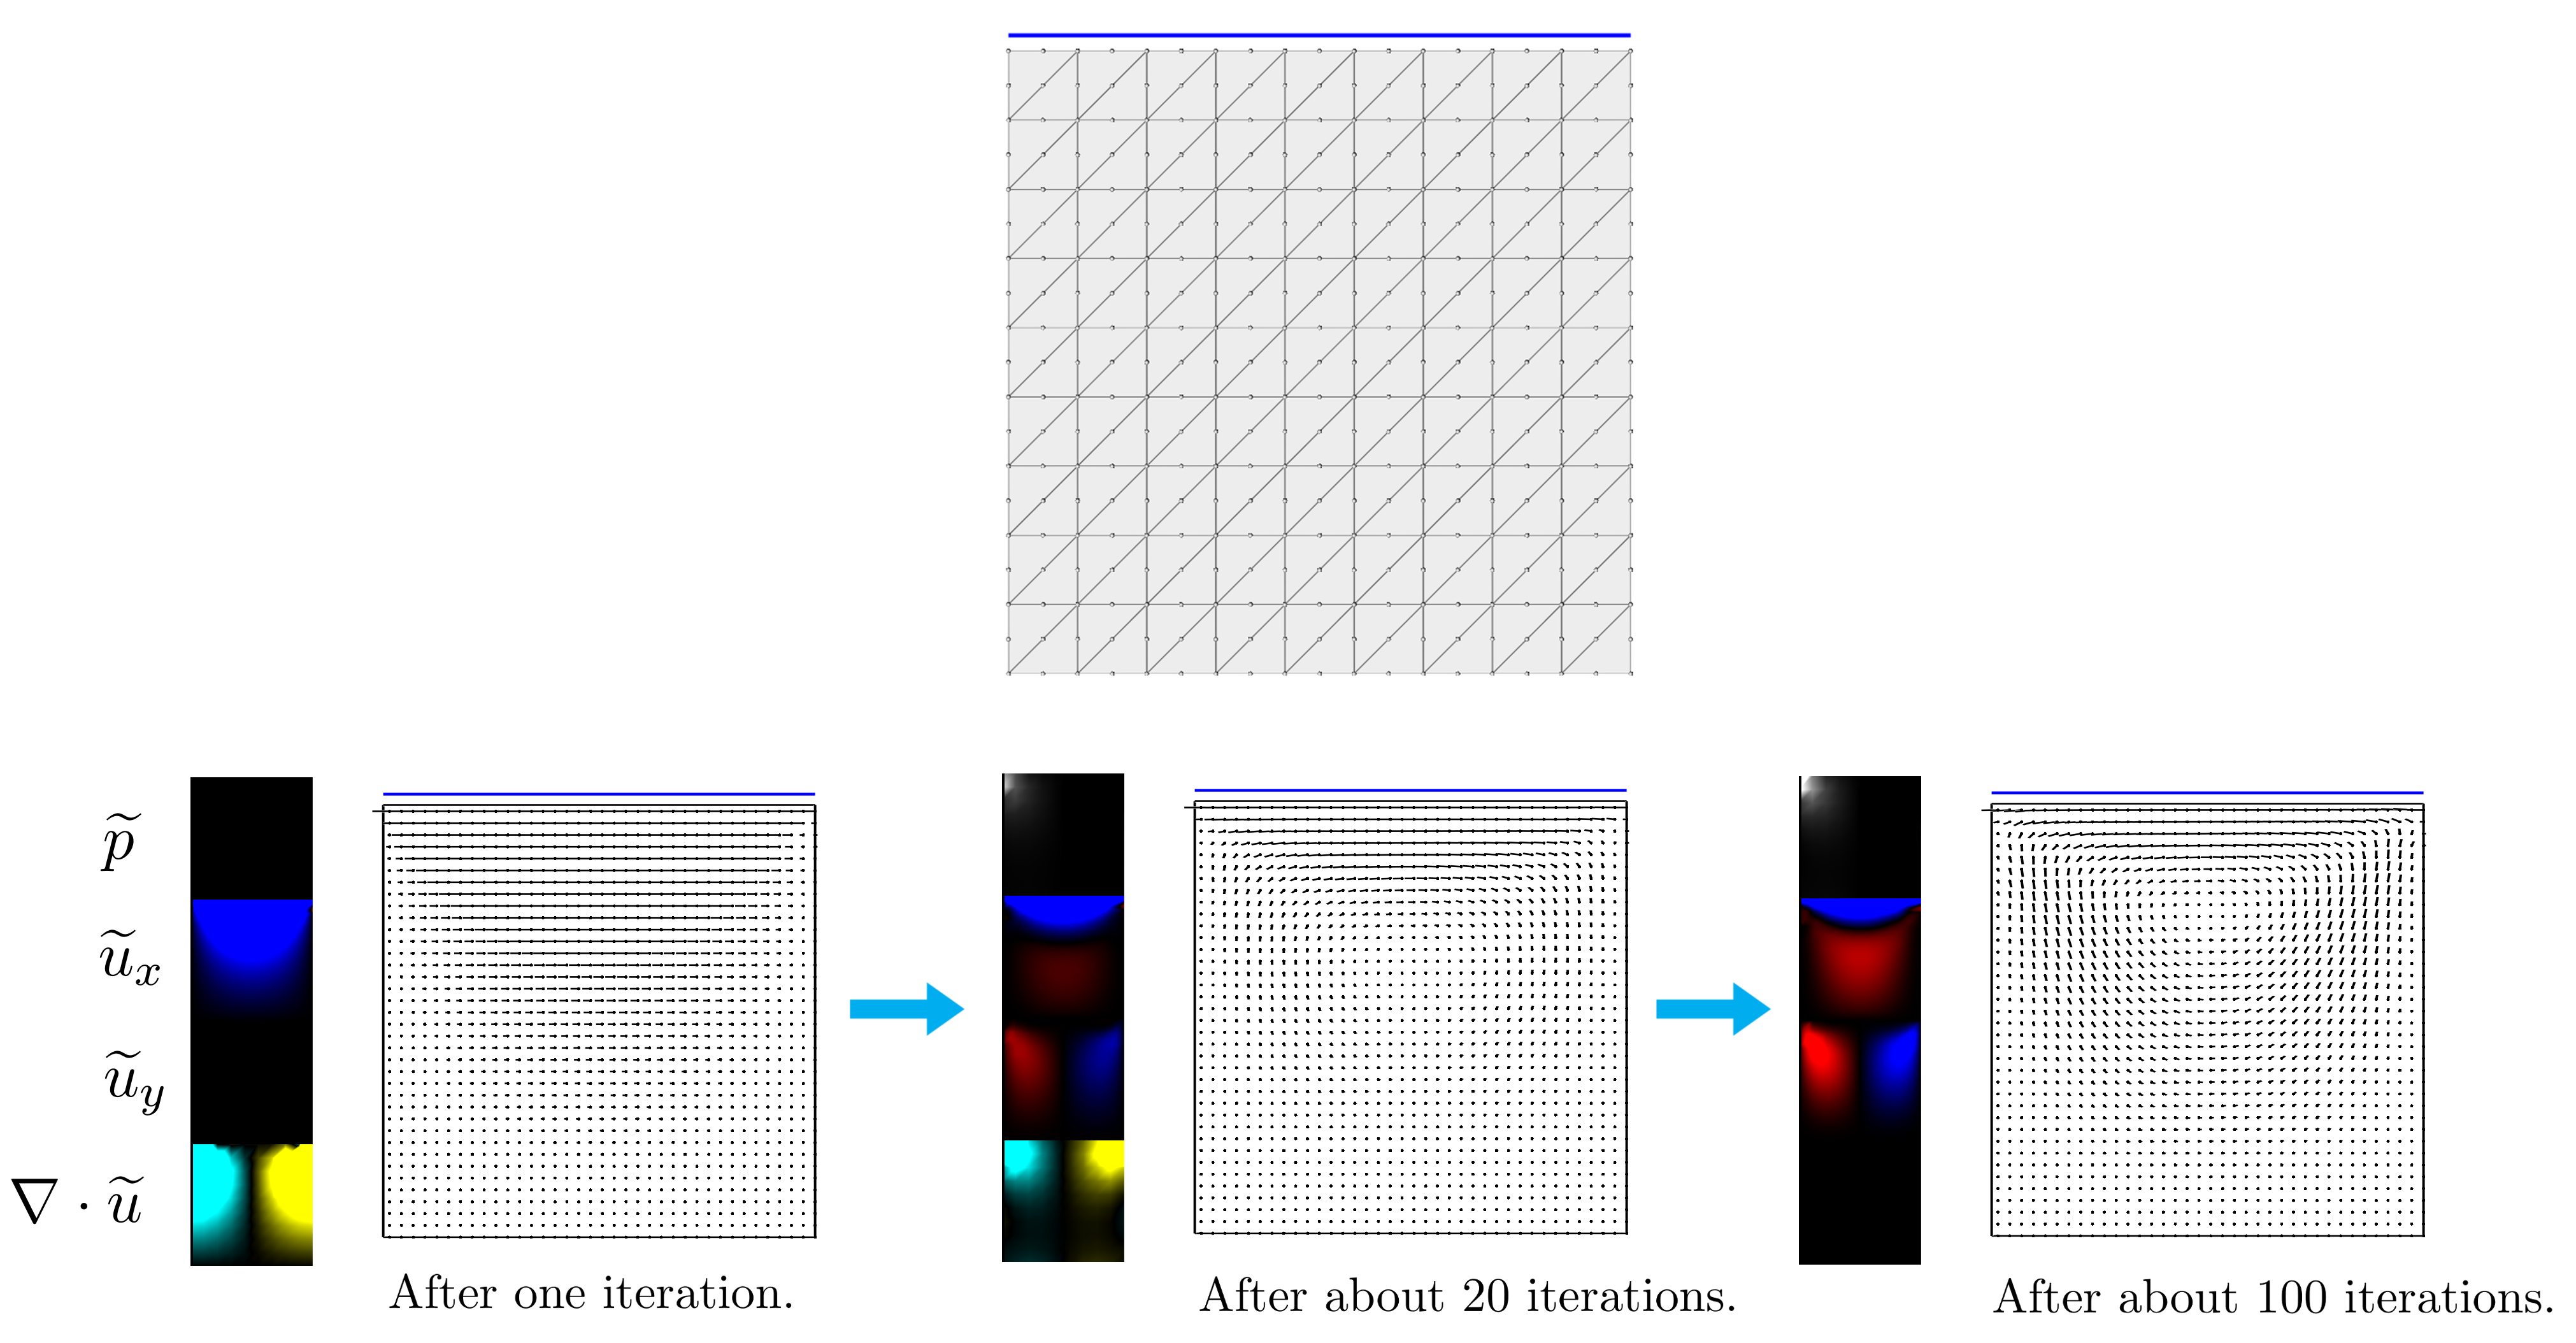
\includegraphics[width=1.3\textwidth]{figures/stokes/lid_driven_weakly_incompressible/figure.png}}
    \label{stokes_lid_driven_weakly_incomprssible}
\end{figure}
This has taken quite a large number of iterations, each iteration solving two large sparse linear systems (the Gramian system being the cheaper to solve).
However, the result is as expected, and this method is easy to implement given an already-working quadratic-element Poisson solver.
However, as implemented, this method is neither general enough nor fast enough to form the basis of a Navier-Stokes solver.


% We will begin by discretizing the \textit{unconstrained} steady Stokes equations,
% which are a vector Poisson equation:
% \begin{equation}\label{steady_stokes_unconstrained}
%     -\mu\Delta u = \rho g.
% \end{equation}
% % >>>
% \subsection{Discretizing the vector Poisson equation}\label{discretizing_vector_poisson}
% % <<<
% In principle we should keep the Stokes equation
% in integral form (using the conservative-form Cauchy momentum equation \eqref{cauchy_continuity_eulerian}), and continue as we did
% in section \ref{trial_function}. However,
% we will take a formal step to skip the reasoning of section \ref{trial_function}, typical of finite element method derivations.
% As we start with the \textit{differential} equation \eqref{steady_stokes_unconstrained}, we can introduce a trial space $\Psi$ and then ``weaken''
% the equation by integrating against $v \in \Psi$, and removing the Laplacian by integration by parts:
% \begin{equation}\label{steady_stokes_unconstrained_weak}
%     \int_\Omega -\mu\Delta u\cdot v\,dx = \int_\Omega \rho g\cdot v\,dx
%     \quad\equiv\quad
%     \int_\Omega -\mu\nabla u : \nabla v\,dx = \int_\Omega \rho g\cdot v\,dx.
% \end{equation}

% Noting that the left-hand-side of \eqref{steady_stokes_unconstrained_weak} is a bilinear form in $u$ and $v$, and the right-hand-side
% is a linear functional in $\psi$, it is standard practice (ref) to write this kind of equation as
% \begin{equation}
%     a(u, v) = f(v).
% \end{equation}
% Our subsequent derivations are much the same as in \ref{discretizing_poisson}, simplified by our new notation.
% We can now approximate $u$ in the test space $\Phi$ as $\hat{u} = \sum_{i=1}^nu_i\phi_i$. By linearity we only need to compute
% trials over the basis trial functions $\psi_j$.
% We then have the linear system of equations
% \begin{equation}\label{elliptic_bilinear_form}
%     \sum_{i=1}^n u_i a\left(\phi_i, \psi_j\right) = f(\psi_j),\quad j=1,\cdots,n,
% \end{equation}
% which can be written in matrix form as
% \begin{equation}\label{elliptic_bilinear_form_matrix}
%     A\hat{u} = \begin{bmatrix}
%             a(\phi_1, \psi_1) & \cdots & a(\phi_1, \psi_n) \\
%             \vdots & & \vdots \\
%             a(\phi_n, \psi_1) & \cdots & a(\phi_n, \psi_n)
%             \end{bmatrix}
%     \begin{bmatrix} u_1 \\ u_2 \\ \vdots \\ u_{n-1} \\ u_n \end{bmatrix}
%     =
%     \begin{bmatrix} f(\psi_1) \\ f(\psi_2) \\ \vdots \\ f(\psi_{n-1}) \\ f(\psi_{n}) \end{bmatrix}
%     = \hat{f}.
% \end{equation}
% % The matrix $A$ is symmetric positive-definite, and we can therefore think of a solution to \eqref{elliptic_bilinear_form_matrix}
% % as as a minimizer of the scalar quadratic form
% % \begin{equation}\label{elliptic_quadratic_form}
% %     \hat{E}(\hat{u}) \coloneqq \frac{1}{2} \inner{\hat{u}, A\hat{u}} - \inner{\hat{u}, \hat{f}}.
% % \end{equation}
% % This is simply a discrete realisation of the fact that we can, as described in section \ref{pressure_derivation}, think
% % of a solution to the vector Poisson equation as a minimizer of the Dirichlet energy \eqref{steady_stokes_dirichlet_energy},
% % \begin{align*}
% %     E(u) \coloneqq \int_{\Omega} \frac{\mu}{2} \inner{\nabla u, \nabla u} - \rho g\cdot u \,dx.
% % \end{align*}
% We can solve \eqref{elliptic_bilinear_form_matrix} to get a velocity field $\sum_{i=1}^n u_i\phi_i$, although in general this will not satisfy $\nabla\cdot u = 0$.
% As some preliminary analysis, if $\Phi = \Psi$ and have the same basis functions, we have a symmetric-positive-definite system. This form of linear system is known to be stably solvable,
% for example by the conjugate gradient method.
% >>>

\section{A mixed finite element method}
As described in section \ref{pressure_derivation}, the pressure $p$ is a Lagrange multiplier that appears
when solving the optimization problem \eqref{stokes_flow_optimization}:
\begin{equation*}
\begin{aligned}
& \underset{u}{\text{minimize}}
& & E(u) =  \frac{\nu}{2} \inner{\nabla u, \nabla u} - \inner{u, \rho g}\\
& \text{subject to}
& & \nabla\cdot u = 0.
\end{aligned}
\end{equation*}

\newcommand{\trialconstraint}{{\Psi_{\text{constraint}}}}
\newcommand{\testpressure}{{\Phi_{\text{pressure}}}}
It is natural, then, to introduce $p$ as a variable to solve for. Solving for the pressure (the ``dual variable'') simultaneously with the velocity
(the ``primal variable'')
is called a primal-dual method for the optimization \eqref{stokes_flow_optimization}, and the resulting finite element method is called \textit{mixed}.

\subsubsection{The pressure finite element space}
Pressure then needs to be discretized, so we introduce another test space $\Phi^p$.
To get a weak form of the steady Stokes equations \eqref{steady_stokes}, including the constraint $-\nabla\cdot u = 0$
(where the negative sign is introduced in order to introduce some structure to the resulting linear system, apparent later), we introduce
another trial space $\Psi^p$, whose functions will be integrated against $-\nabla\cdot u$.

\subsubsection{The velocity finite element product space }
Further, we introduce a $2n_u$--dimensional vector finite element space for velocity as a trivial product of scalar finite element spaces:
$$
    \Phi^u = \Phi^{u,s} \times \Phi^{u,s}.
$$
A natural choice for the basis functions of $\Phi^u$ is:
    $$\Phi^u = \text{span}\left\{\phi_1^{u,s}\partial x, \phi_1^{u,s}\partial y,
    \cdots,
    \phi_{n_u}^{u,s}\partial x, \phi_{n_u}^{u,s}\partial y
\right\},$$
where $\partial x$ and $\partial y$ denote unit vector fields in the axis directions.

\subsection{The mixed weak form of the steady Stokes equations}
The weak form is then
\begin{equation*}
\begin{split}
    &\int_\om \left(-\nu\Delta u + \nabla p\right)\cdot \psi^u\,dx = \int_\Omega \rho g\cdot\psi^u\,d\hat{x},\\
    &\int_\om -\psi^p\left(\nabla\cdot u\right)\,d\hat{x} = 0, \quad\text{where $\psi^u \in \Psi^u, \psi^p \in \Psi^p$},
\end{split}
\end{equation*}
which by integration by parts can be written as
\begin{equation}\label{steady_stokes_weak}
\begin{split}
    &\int_\om \nu\nabla u : \nabla \psi^u - p\nabla\cdot \psi^u\,d\hat{x} = \int_\om \rho g \cdot \psi^u\,d\hat{x},\\
    &\int_\om -\psi^p\left(\nabla\cdot u\right)\,d\hat{x} = 0, \quad\text{where $\psi^u \in \Psi^u, \psi^p \in \Psi^p$},
\end{split}
\end{equation}
This can be thought of as a single equation integrated against basis functions in the ``mixed'' finite element spaces
    $$\Phi^\mathcal{M} = \Phi^u \times \Phi^p \text{\quad and \quad} \Psi^\mathcal{M} = \Psi^u \times \Psi^p$$
with basis functions
\begin{equation}\label{mixed_space_basis_functions}
\begin{split}
    \Phi^\mathcal{M} &= \text{span}\left\{
        (\phi^u_1, 0),\cdots,(\phi^u_n, 0), (0,\phi_1^p),\cdots,(0,\phi_n^p)
    \right\},\\
    \Psi^\mathcal{M} &= \text{span}\left\{
        (\psi^u_1, 0),\cdots,(\psi^u_n, 0), (0,\psi_1^p),\cdots,(0,\psi_n^p)
    \right\}.
\end{split}
\end{equation}
We will not use this formalism, but it is helpful when automating the finite element method \cite{automating_fem}.
This mixed space forms the ``Taylor-Hood elements'', and is known to result in a stable method for the Stokes problem \footnote{
While we could choose just about any spaces for the non-mixed method for the Poisson problem, which is elliptic, the Stokes flow problem
inherently involves a Lagrange multiplier, and is known as a ``saddle point problem''. The resulting finite element matrix is hyperbolic.
The Taylor-Hood elements satisfy the Ladyzhenskaya--Babu\v ska--Brezzi (LBB) condition, which
is a theoretical result which guarantees that the resulting linear system for the Stokes problem will be well-conditioned.
If we took $P^1 \times P^1$ instead, for example, this condition would not hold.
}.

% So we don't have to repeat the equations for each kind of mixed trial function, as we do in \eqref{stokes_flow_mixed_equations_1}, we can use the mixed basis order \eqref{mixed_space_basis_functions} and define $\phi^\mathcal{M}_l$ to be the $l$'th mixed basis
% function in this order (e.g. $\psi^\mathcal{M}_1 = (\psi_1, 0)$ and $\psi^\mathcal{M}_{n+1} = (0, \psi^p_1)$).
% 
% \begin{aside}
% \textit{A note on tensor notation for the vector field space}
% \vskip 0.1in
% 
% The space $P^2_2$ here is a space of piecewise quadratic vector fields formed as $P^2_2 = P^2 \times P^2$.
% This represents the velocity field by two functions in the usual scalar quadratic space $P^2$.
% This is the simplest way to construct a finite element space of vector fields, although others (not based on a product construction) are possible.
% We define $\partial x$ and $\partial y$ to be the unit vector fields on the domain $\Omega$.
% The basis functions for $P^2_2$ are the natural choice of vector fields $\phi^\text{scalar}_1\partial x$, $\phi^\text{scalar}_1\partial y$, $\cdots$, $\phi^\text{scalar}_n\partial x$, $\phi^\text{scalar}_n\partial y$.
% However, we would like to think of the velocity coefficients as vector samples, rather than scalar coefficients
% of this array of $2n$ basis vector fields. We can do this by letting $\phi_1,\cdots,\phi_n$ be aggregates of axis-aligned vector fields:
%     $$
%         \phi_i = \begin{bmatrix}
%         \phi_{ix} \coloneqq \phi^\text{scalar}_{i}\partial x\\
%         \phi_{iy} \coloneqq \phi^\text{scalar}_{i}\partial y\end{bmatrix}.
%     $$
% We can then represent the interior variation as
%     $$\tilde{u}_\text{interior} = \sum_{i=1}^n u_i \cdot \phi_i.$$
% It is important to keep this in mind, as although this notation is natural, it may cause confusion:
% While $a$ is a bilinear form, the value $a((\phi_1, 0), \psi^\mathcal{M}_4)$, for example, is actually ``vectorized''
% into
%     $$
%         \begin{bmatrix}
%             a((\phi_{1x}, 0), \psi^\mathcal{M}_4)\\
%             a((\phi_{1y}, 0), \psi^\mathcal{M}_4)
%         \end{bmatrix}.
%     $$
% This is contracted with the vector coefficient $u^1$ to get a scalar:
%     $$
%         u^1 \cdot a((\phi_1, 0), \psi^\mathcal{M}_4)
%     = u^1_x a((\phi_{1x},0), \psi^\mathcal{M}_4)
%         + u^1_y a((\phi_{1y},0), \psi^\mathcal{M}_4).
%     $$
% \end{aside}

\subsection{Forming a linear system from the mixed weak form}
Let $u$ be approximated by
    $$\tilde{u} = \tilde{u}_\Gamma + \tilde{u}_\text{interior} = \tilde{u}_\Gamma + \sum_{i=1}^n u_i\cdot \phi_i,$$
where $\tilde{u}_\Gamma \in \Phi^{*,u}$ approximates the Dirichlet boundary function $\left.u\right|_\Gamma = u_\Gamma$,
and $\tilde{u}_{\text{interior}} \in \Phi^u$ is the ``interior variation''.
$\Phi^{*,u}$ is the full P2 vector finite element space, which is not required to be zero on the boundary.
A boundary condition for pressure is not given. Pressure is approximated as
    $$\tilde{p} = \sum_{i=1}^n p_i\phi^p_i.$$
Now, substituting $u \leftarrow \tilde{u}$ and $p \leftarrow \tilde{p}$, the mixed weak form \eqref{steady_stokes_weak} expands to,
rearranging constants to the right-hand side,
\begin{equation}\label{steady_stokes_linear_system}
\begin{split}
&\sum_{i=1}^n \left[u_i\cdot \int_\Omega -\mu\nabla\phi_i : \nabla\psi_j\,d\hat{x}
        + p_i\int_{\Omega} -\psi_j \cdot \nabla\phi_{pi}\,d\hat{x}\right]
    = \int_\Omega \rho g\cdot\psi_j
        + \mu\nabla\phi_\Gamma :\nabla\psi_j \,d\hat{x},\\
&\sum_{i=1}^n u_i \cdot \int_\Omega -\phi_i \cdot \nabla q_j \,d\hat{x}
    = \int_\Omega \phi_\Gamma \cdot \nabla q_j \,d\hat{x},
\quad\quad j=1,\cdots,n.
\end{split}
\end{equation}

\begin{figure}[H]
    \centering
    \centerline{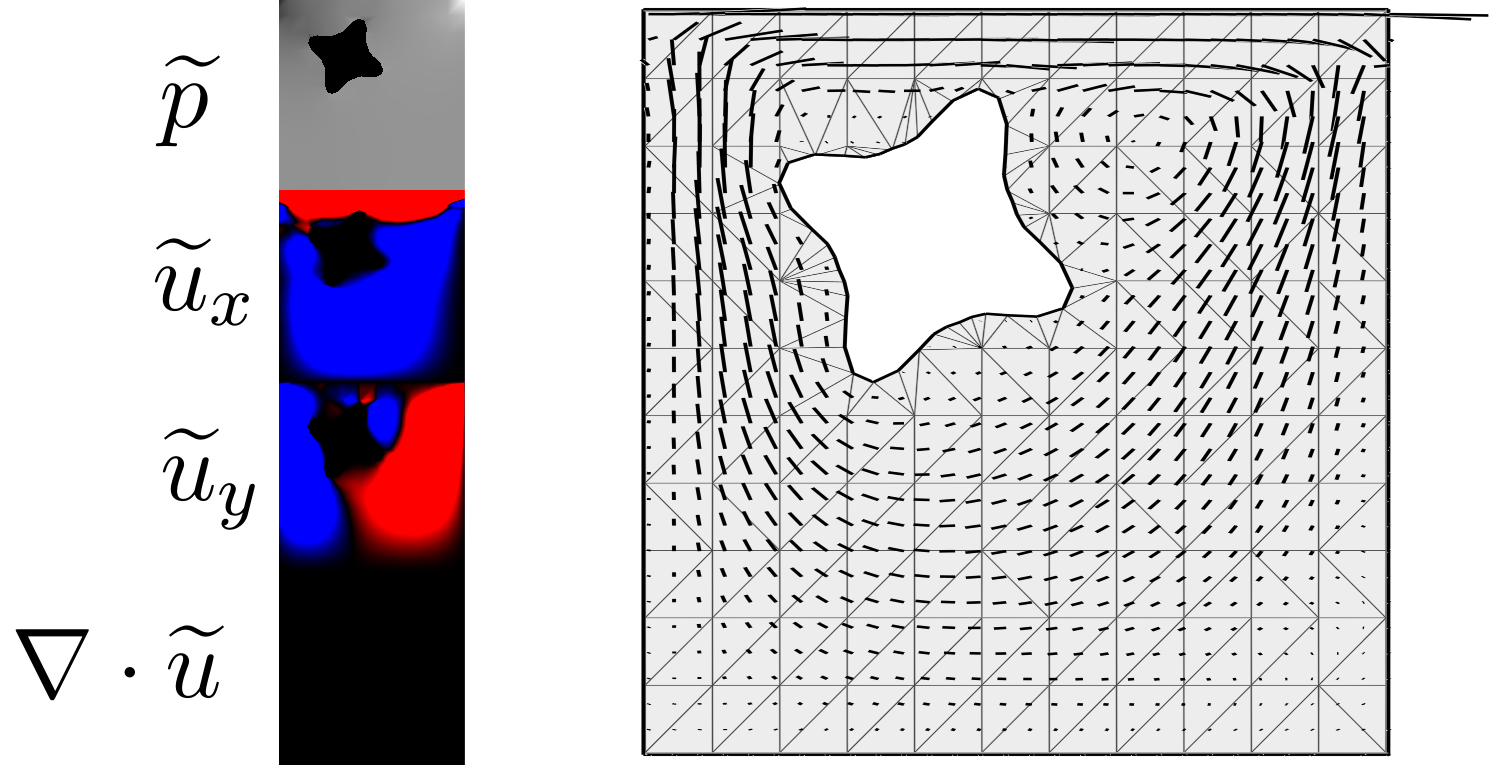
\includegraphics[width=0.8\textwidth]{figures/stokes/lid_driven_obstruction/figure.png}}
    \label{stokes_lid_driven_obstruction}
\end{figure}


% \begin{align*}
%     &\widetilde{u}_x\\
%     &\widetilde{u}_y\\
%     &\widetilde{p}\\
%     &\nabla\cdot \widetilde{u}
% \end{align*}
% 
% After one iteration.
% 
% After about 20 iterations.
% 
% After about 100 iterations.
